%\graphicspath{{~/Pictures/Screenshots/}}
\graphicspath{{~/Documents/MobAppDev/ThirdTask/img}}
\section*{\LARGE{Цель практической работы}}
\addcontentsline{toc}{section}{Цель практической работы}

\newpage

\section*{\LARGE{Выполнение практической работы}}
\addcontentsline{toc}{section}{Выполнение практической работы}

\section{Основы создания интерфейса}
При запуске приложения сначала запускается класс
MainActivity, который в качестве графического интерфейса устанавливает
разметку из файла activity\_main.xml. И поскольку в этой разметке прописан
элемент TextView, который представляет некоторый текст, то увидим
его текст на экране смартфона.

\subsection{Создание графического интерфейса}
Выполнение приложения Android по умолчанию начинается с класса
MainActivity, который по умолчанию открыт в Android Studio,
пример показан на рисунке \ref{fig:activity:start}.

\begin{figure}[h!tp]
	\centering
	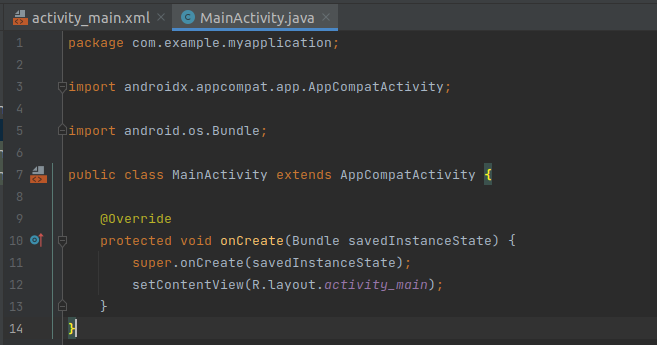
\includegraphics[width=0.6\textwidth]{Screenshot from 2023-03-09 17-16-57.png}
	\caption{Файл MainActivity.java}
	\label{fig:activity:start}
\end{figure}

Каждый отдельный экран или страница в приложении описывается таким
понятием как activity. В литературе могут использоваться различные
термины: экран, страница, активность.
Так вот, если запустить приложение на устройстве, то на экране появиться
определенную activity, которая предсталяет данный интерфейс.\par
Класс MainActivity, по сути, представляет обычный класс java, в начале
которого идет определение пакета данного класса.\par
Далее идет импорт классов из других пакетов, функциональность которых
используется в MainActivity.\par
По умолчанию MainActivity содержит только один метод \texttt{onCreate()}, в
котором фактически и создается весь интерфейс приложения.
В нем вызывается метод \texttt{setContentView()} передается ресурс разметки
графического интерфейса.
Именно здесь и решается, какой именно визуальный интерфейс будет иметь
MainActivity. Ресурс \texttt{R.layout.activity\_main} --- это файл
activity\_main.xml из каталога res/layout (в
принципе можно заметить, что название ресурса соответствует названию
файла), который также по умолчанию открыт в Android Studio.

\subsection{Файл activity\_main.xml}
Android Studio позволяет работать с визуальным интерфейсом как в режиме
кода, так и в графическом режиме. Так, по умолчанию файл открыт в
графическом режиме, и можно наглядно увидеть, как у примерно
будет выглядеть экран приложения.
Но также можно работать с файлом в режиме кода, поскольку
activity\_main.xml --- это обычный текстовый файл с разметкой xml. Для
переключения к коду нужно нажать на кнопку Code над графическим
представлением.\par
Разметка на уровне кода файл activity\_main.xml изображена
на рисунке \ref{fig:xml:layout}.

\begin{figure}[h!tp]
	\centering
	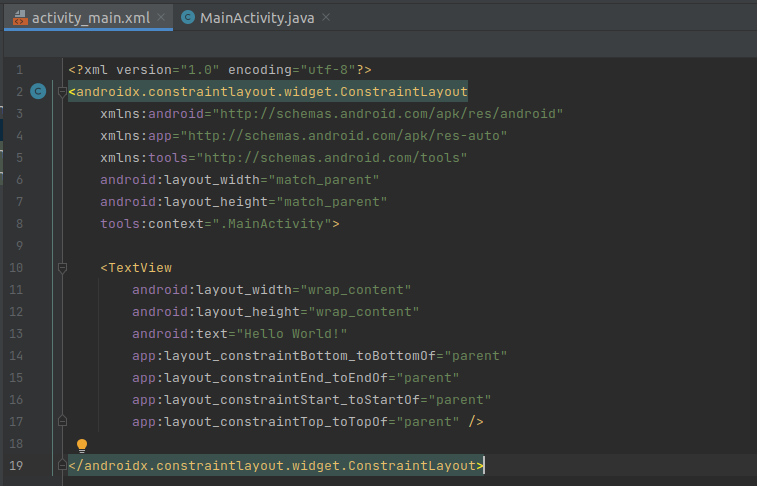
\includegraphics[width=0.8\textwidth]{Screenshot from 2023-03-09 17-29-58.png}
	\caption{Пример содержимого файла разметки}
	\label{fig:xml:layout}
\end{figure}

Весь интерфейс представлен элементом-контейнером
\texttt{androidx.constraintlayout.widget.ConstraintLayout}.\par
ConstraintLayout позволяет расположить вложенные элементы в
определенных местах экрана. Вначале элемента ConstraintLayout идет
определение пространств имен XML.
Каждое пространство имен задается следующим образом:
\texttt{xmlns:префикс="название\_ресурса"}.\par
Название ресурса (или URI - Uniform Resource Indicator) ---
\texttt{"http://schemas.android.com/apk/res/android"}.
И этот ресурс сопоставляется с префиксом android (\texttt{xmlns:android}).\par
Каждый ресурс или URI определяет некоторую функциональность,
которая используется в приложении, например, предоставляют теги и атрибуты,
которые необходимые для построения приложения:
\begin{itemize}
	\item \texttt{xmlns:android="http://schemas.android.com/apk/res/android"}:
		содержит основные атрибуты, которые предоставляются платформой
		Android, применяются в элементах управления и определяют
		их визуальные свойства (например, размер, позиционирование)
	\item \texttt{xmlns:app="http://schemas.android.com/apk/res-auto"}:
		содержит атрибуты, которые определены в рамках приложения
	\item \texttt{xmlns:tools="http://schemas.android.com/tools"}:
		применяется для работы с режиме дизайнера в Android Studio
\end{itemize}

И чтобы упростить работу с этими ресурсами, применяются префиксы.\par
\texttt{android:layout\_width} определяет ширину контейнера. Этот атрибут
(layout\_width) расположен в ресурсе
"http://schemas.android.com/apk/res/android". И поскольку этот ресурс
сопоставляется с префиксом android, то для обращения к атрибуту перед ним
через двоеточие указывается префикс данного ресурса.\par
Значением атрибута \texttt{android:layout\_weight} является
"match\_parent". Это значит, что элемент (ConstraintLayout)
будет растягиваться по всей ширине контейнера (экрана устройства).\par
Атрибут \texttt{android:layout\_height="match\_parent"} определяет высоту
контейнера и также определен в
"http://schemas.android.com/apk/res/android".\par
Значение "match\_parent" указывает, что ConstraintLayout
будет растягивается по всей длине контейнера (экрана устройства).\par
Атрибут \texttt{tools:context} определяет, какой класс
activity (экрана приложения) связан с текущим определением интерфейса.
В данном случае это класс MainActivity. Это позволяет использовать
в Android Studio различные возможности в режиме дизайнера,
которые зависят от класса activity.

\subsection{TextView}
Текстовое поле устанавливает текст с помощью атрибута android:text
(Рисунок \ref{fig:xml:textview}).

\begin{figure}[h!tp]
	\centering
	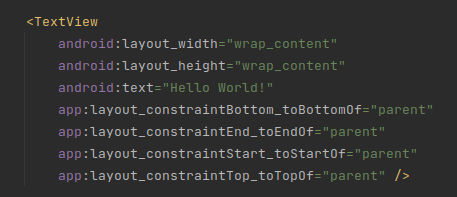
\includegraphics[width=0.8\textwidth]{Screenshot from 2023-03-09 17-49-55.png}
	\caption{Пример кода виджета TextView}
	\label{fig:xml:textview}
\end{figure}

\begin{description}
	\item[android:layout\_width] устанавливает ширину виджета. Значение
		wrap\_content задает для виджета величину, достаточную для
		отображения в контейнере.
	\item[android:layout\_height] устанавливает высоту виджета. Значение
		wrap\_content аналогично установке ширины задает для виджета высоту,
		достаточную для отображения в контейнере
	\item[android:text] устанавливает текст, который будет выводиться
		в TextView (в данном случае это строка "Hello World!")
	\item[app:layout\_constraintLeft\_toLeftOf="parent"] указывает, что левая
		граница элемента будет выравниваться по левой стороне контейнера
		ConstraintLayout
	\item[app:layout\_constraintTop\_toTopOf="parent"] указывает, что верхняя
		граница элемента будет выравниваться по верхней стороне контейнера
		ConstraintLayout
	\item[app:layout\_constraintRight\_toRightOf="parent"] указывает,
		что правая граница элемента будет выравниваться по правой стороне
		контейнера ConstraintLayout
\end{description}

\section{Создание интерфейса в коде java}
Для работы с визуальными элементами создадим новый проект. В качестве
шаблона проекта выберем Empty Activity.\par
Определим в классе MainActivity простейший интерфейс
(Рисунок~\ref{fig:activity:layout:java}).

\begin{figure}[h!tp]
	\centering
	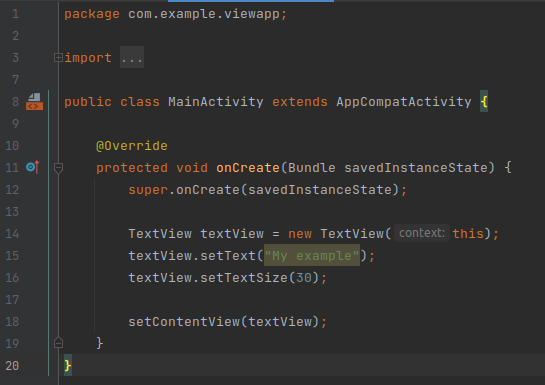
\includegraphics[width=0.8\textwidth]{Screenshot from 2023-03-09 18-10-05.png}
	\caption{Реализация интерфейса на джава}
	\label{fig:activity:layout:java}
\end{figure}

При создании виджетов в коде Java применяется их конструктор, в который
передается контекст данного виджета, а точнее объект
android.content.Context, в качестве которого выступает текущий класс
MainActivity.\par
Здесь весь интерфейс представлен элементом TextView, которое
предназначено для выводa текста. С помощью методов, которые, как
правило, начинаются на set, можно установить различные свойства TextView.
Например, в данном случае метод setText() устанавливает текст в поле, а
setTextSize() задает высоту шрифта.\par
Для установки элемента в качестве интерфейса приложения в коде Activity
вызывается метод setContentView(), в который передается визуальный
элемент.\par
Если запустить приложение, то получится визуальный интерфейс, показанный
на рисунку~\ref{fig:view:textview:java}.

\begin{figure}[h!tp]
	\centering
	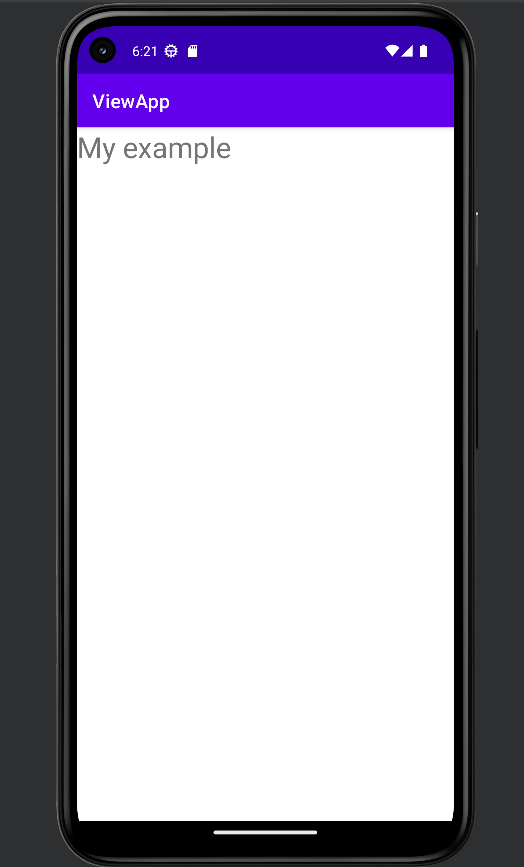
\includegraphics[width=0.8\textwidth]{Screenshot from 2023-03-09 18-21-21.png}
	\caption{Реализация интерфейса на джава}
	\label{fig:view:textview:java}
\end{figure}

\section{Определение интерфейса в файле XML}
Как правило, для определения визуального интерфейса в проектах под
Android используются специальные файлы xml. Эти файлы являются
ресурсами разметки и хранят определение визуального интерфейса в виде
кода XML. Подобный подход напоминает создание веб-сайтов, когда
интерфейс определяется в файлах html, а логика приложения - в коде
javascript.\par
Объявление пользовательского интерфейса в файлах XML позволяет
отделить интерфейс приложения от кода. Что означает, что мы можем
изменять определение интерфейса без изменения кода java. Например, в
приложении могут быть определены разметки в файлах XML для различных
ориентаций монитора, различных размеров устройств, различных языков и
т.д. Кроме того, объявление разметки в XML позволяет легче
визуализировать структуру интерфейса и облегчает отладку.\par
Файлы разметки графического интерфейса располагаются в проекте в
каталоге res/layout. По умолчанию при создании проекта с пустой activity уже
есть один файл ресурсов разметки activity\_main.xml, который может
выглядеть примерно так, как показано на рисунке~\ref{fig:xml:layout:d}.

\begin{figure}[h!tp]
	\centering
	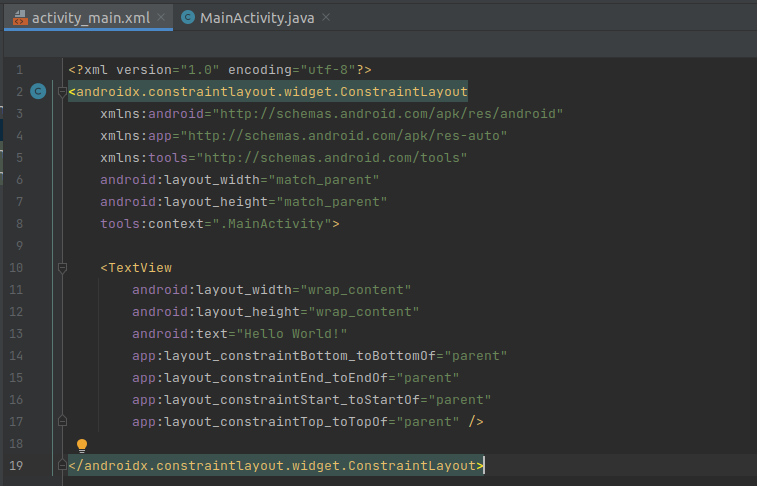
\includegraphics[width=0.8\textwidth]{Screenshot from 2023-03-09 17-29-58.png}
	\caption{Пример содержимого файла разметки}
	\label{fig:xml:layout:d}
\end{figure}
